\section{Durchführung}
\subsection{Theoretischer Teil}

\subsection{Kalibriermessungen}
    \subsubsection{Messung einer Quelle bekannter Aktivität bei mittiger Quellposition}
       Zunächst haben wir eine Quelle in mittigem Abstand zu den beiden Detektoren vermessen. Die Quelle hatte am 29.10.2015 eine Aktivitiät $A = \unit[1,02]{MBq}$.\\
       \vspace{2mm}
        
       \begin{tabular}{p{6cm}p{6cm}l}
               \minipanf 
                   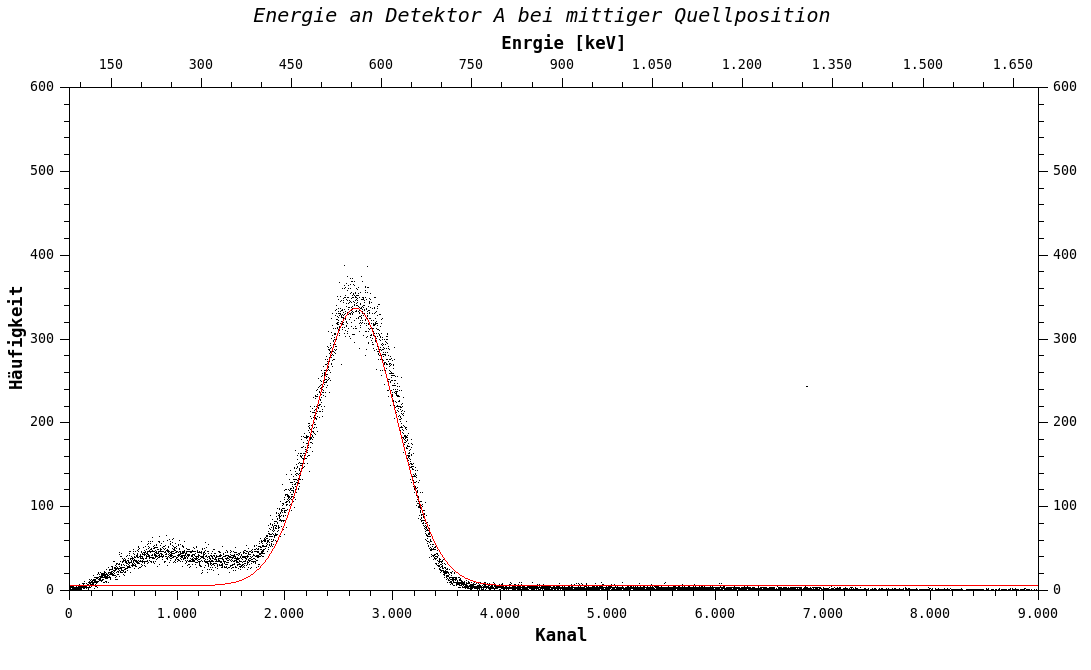
\includegraphics[width=1.2\textwidth, height=0.225\textheight]{pic/Efenster_DetA_M.png}
                   \label{dfd:EdetA_M}
               \minipend
               &
               \hspace{9mm}
               \minipanf 
                   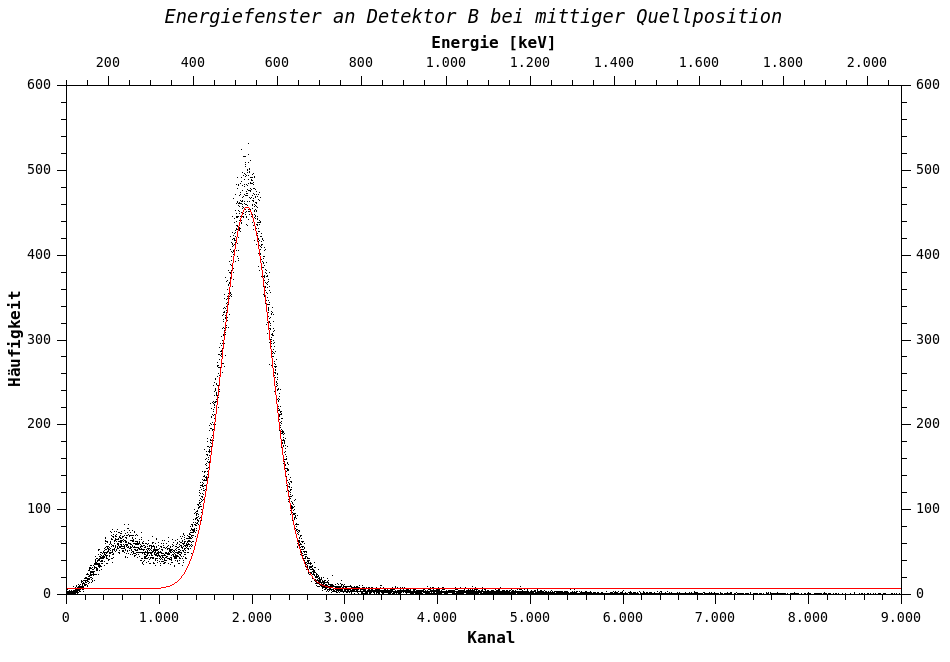
\includegraphics[width=1.2\textwidth, height=0.225\textheight]{pic/Efenster_DetB_M.png}
                   \label{dfd:EdetB_M}
               \minipend\\
               \multicolumn{2}{c}{\hspace{1.5cm}
                   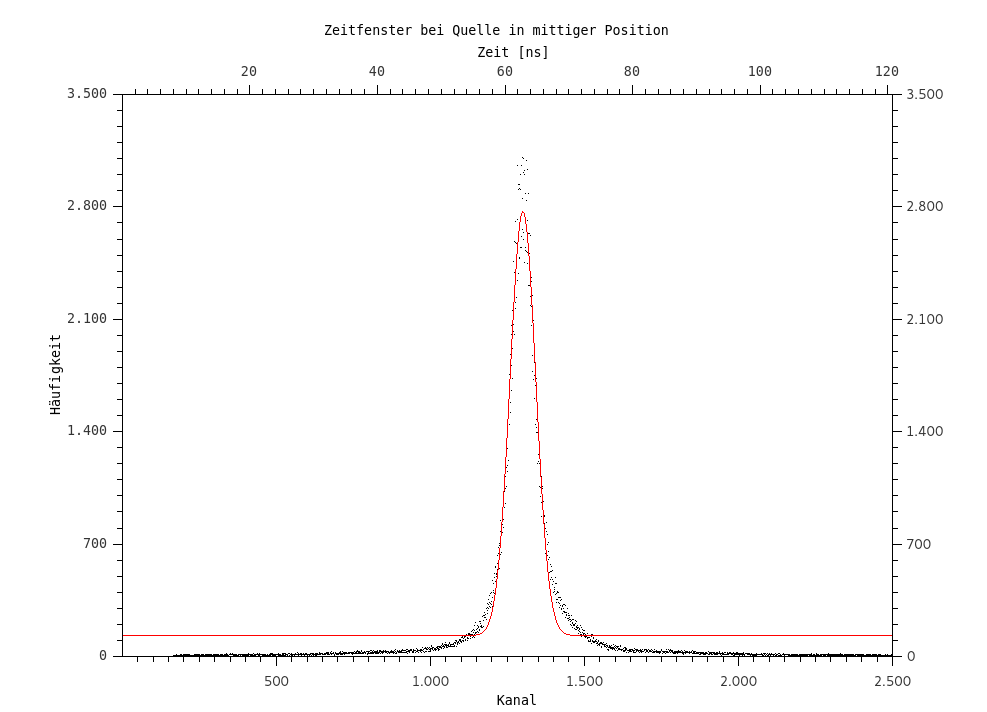
\includegraphics[width=0.7\textwidth, height=0.3\textheight]{pic/T_M_dia.png}
                   \label{dfd:T_M}}\\                        
       \end{tabular}
       \captionof{table}{Kalibrationsmessung bei Quelle mittig zwischen den Detektoren A und B}


    \subsubsection{Messung bei Positionen direkt an den Detektoren}
        \begin{tabular}{p{6cm}p{6cm}l}
            \minipanf 
                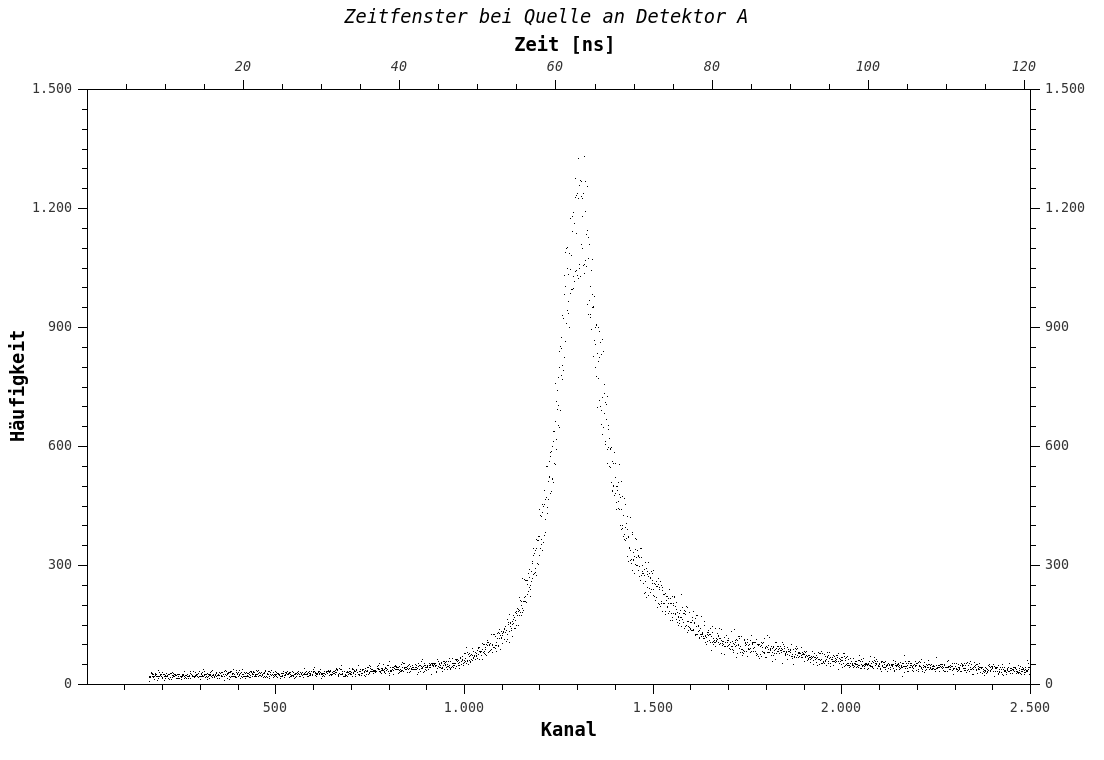
\includegraphics[width=1.2\textwidth, height=0.225\textheight]{pic/T_A_dia.png}
                \label{dfd:T_A}
            \minipend
            &
            \hspace{9mm} 
            \minipanf
                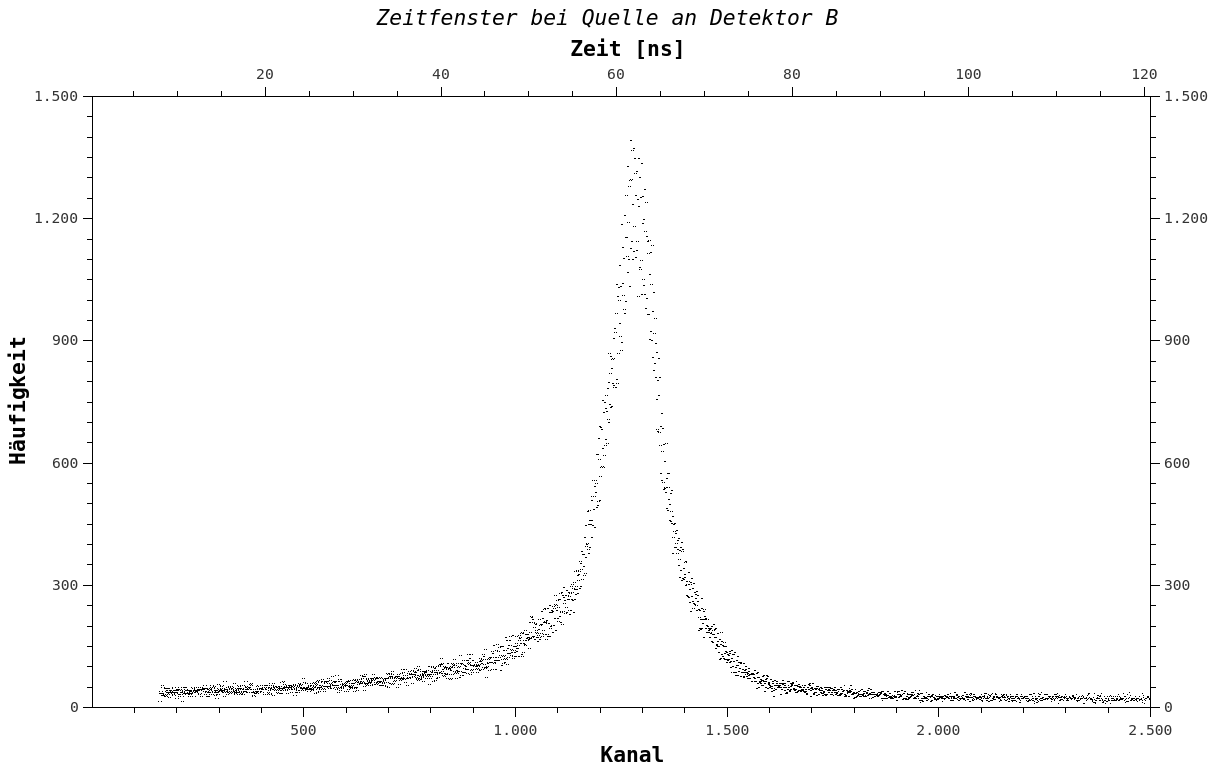
\includegraphics[width=1.2\textwidth, height=0.225\textheight]{pic/T_B_dia.png}
                \label{dfd:T_B}
            \minipend \\
            \minipanf
                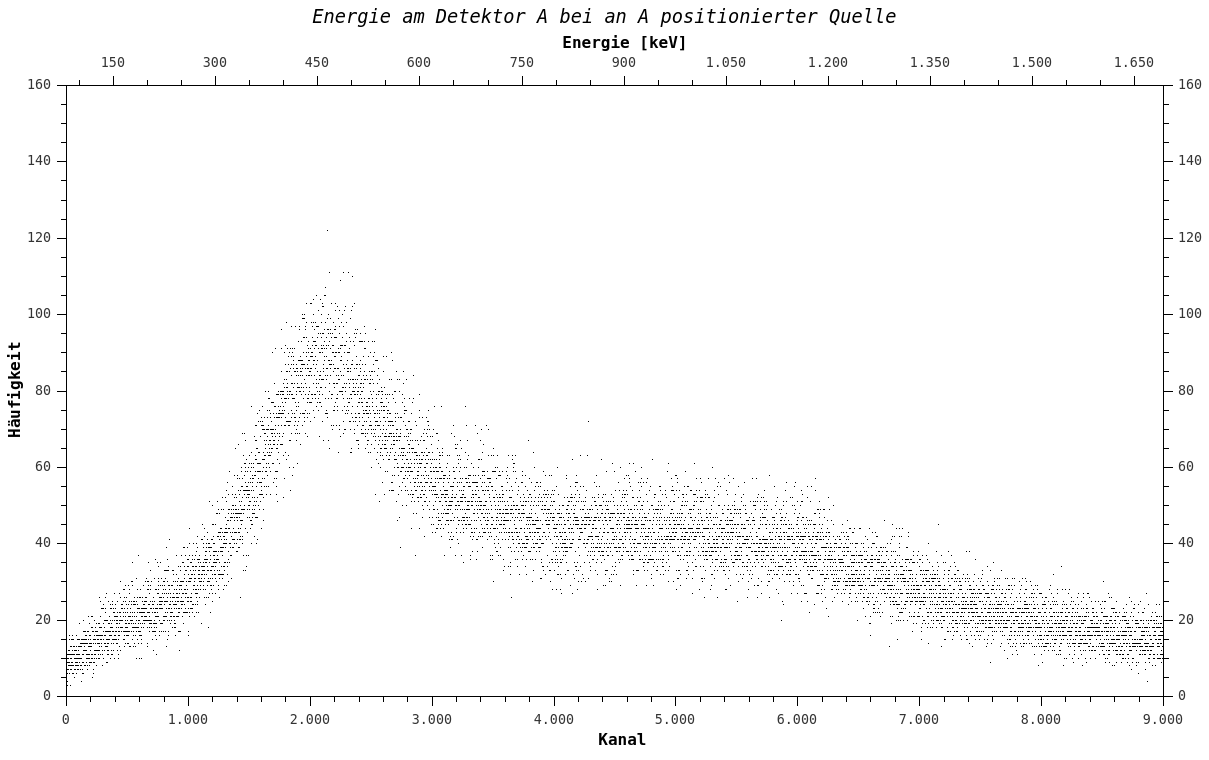
\includegraphics[width=1.2\textwidth, height=0.225\textheight]{pic/Efenster_DetA_A.png}
                \label{dfd:EdetAA}
            \minipend
            &
            \hspace{9mm} 
            \minipanf 
                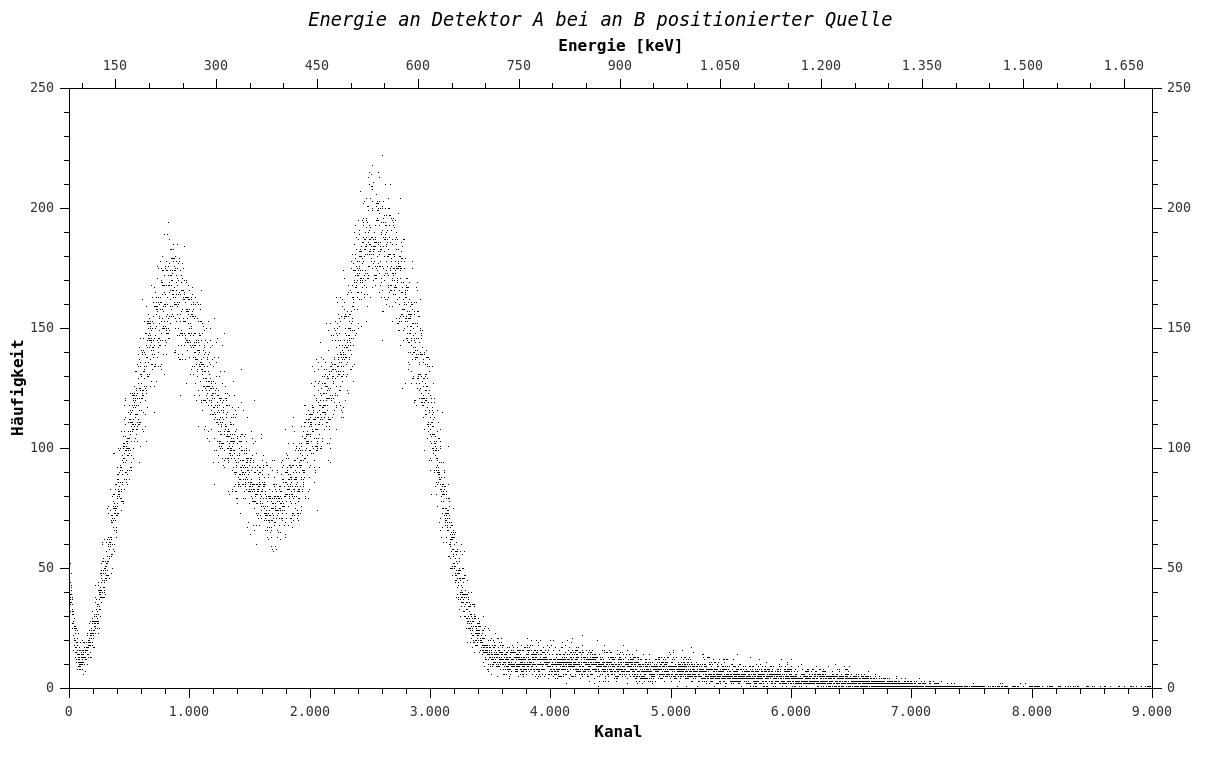
\includegraphics[width=1.2\textwidth, height=0.225\textheight]{pic/Efenster_DetA_B.png}
                \label{dfd:EdetBA}
            \minipend \\
            \minipanf 
                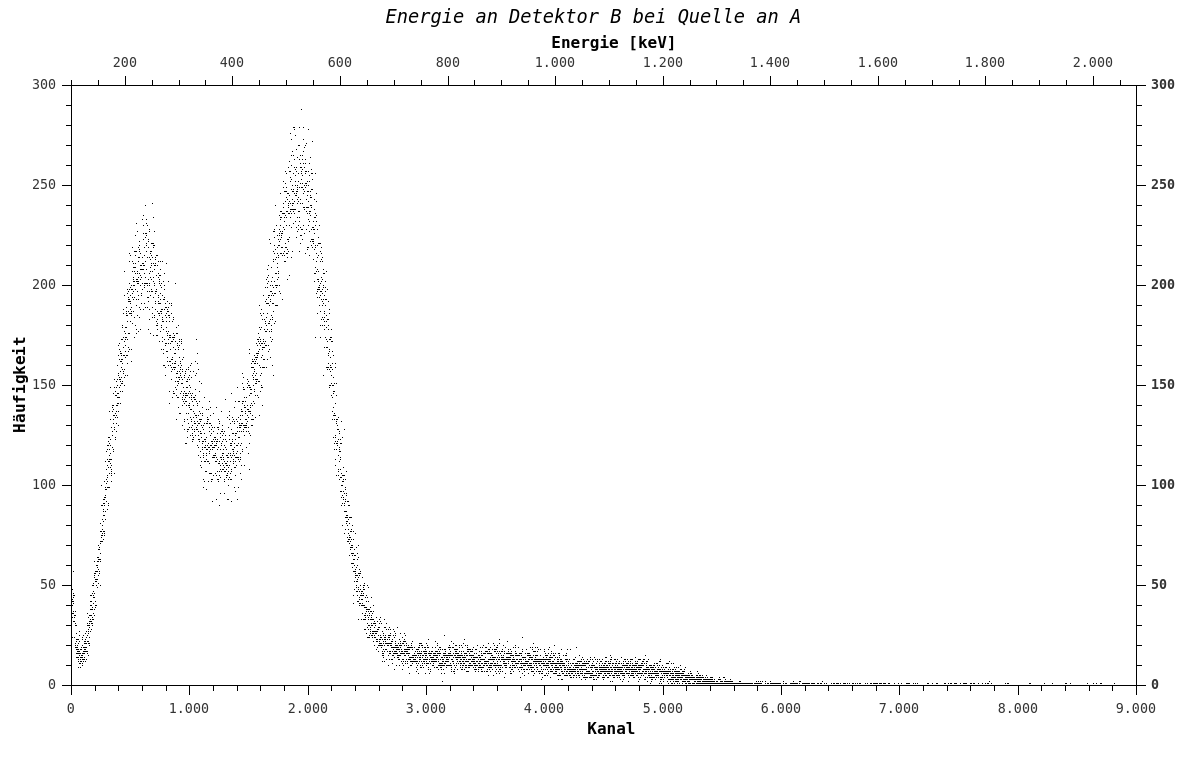
\includegraphics[width=1.2\textwidth, height=0.225\textheight]{pic/Efenster_DetB_A.png}
                \label{dfd:EdetAB}
            \minipend
            &
            \minipanf 
                \hspace{9mm}
                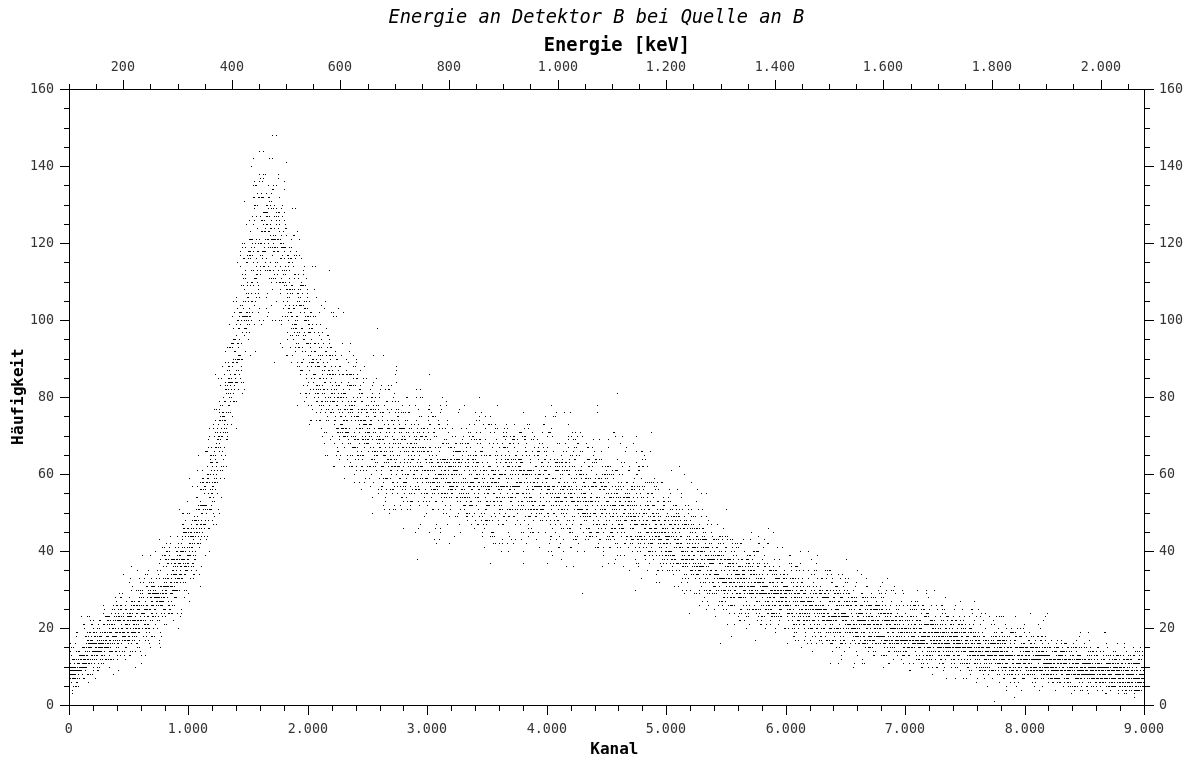
\includegraphics[width=1.2\textwidth, height=0.225\textheight]{pic/Efenster_DetB_B.png}
                \label{dfd:EdetBB}
            \minipend \\            
        \end{tabular}
        \captionof{figure}{Gegenüberstellung der Messungen mit der Quelle an Det. A (links) und Det. B (rechts)} 
        
    \subsection{Tomografische Messungen}
    	\subsubsection{Messung einer Quellkonfiguration, Phantom isotroper Dichteverteilung}
            \textbf{Hauptversuch}\\
            
            \textbf{Untersuchung des Einflusses verschiedener Filter}\\
            
            \begin{tabular}{p{6cm}p{6cm}c}
                            \minipanf 
                                \makebox[\linewidth]{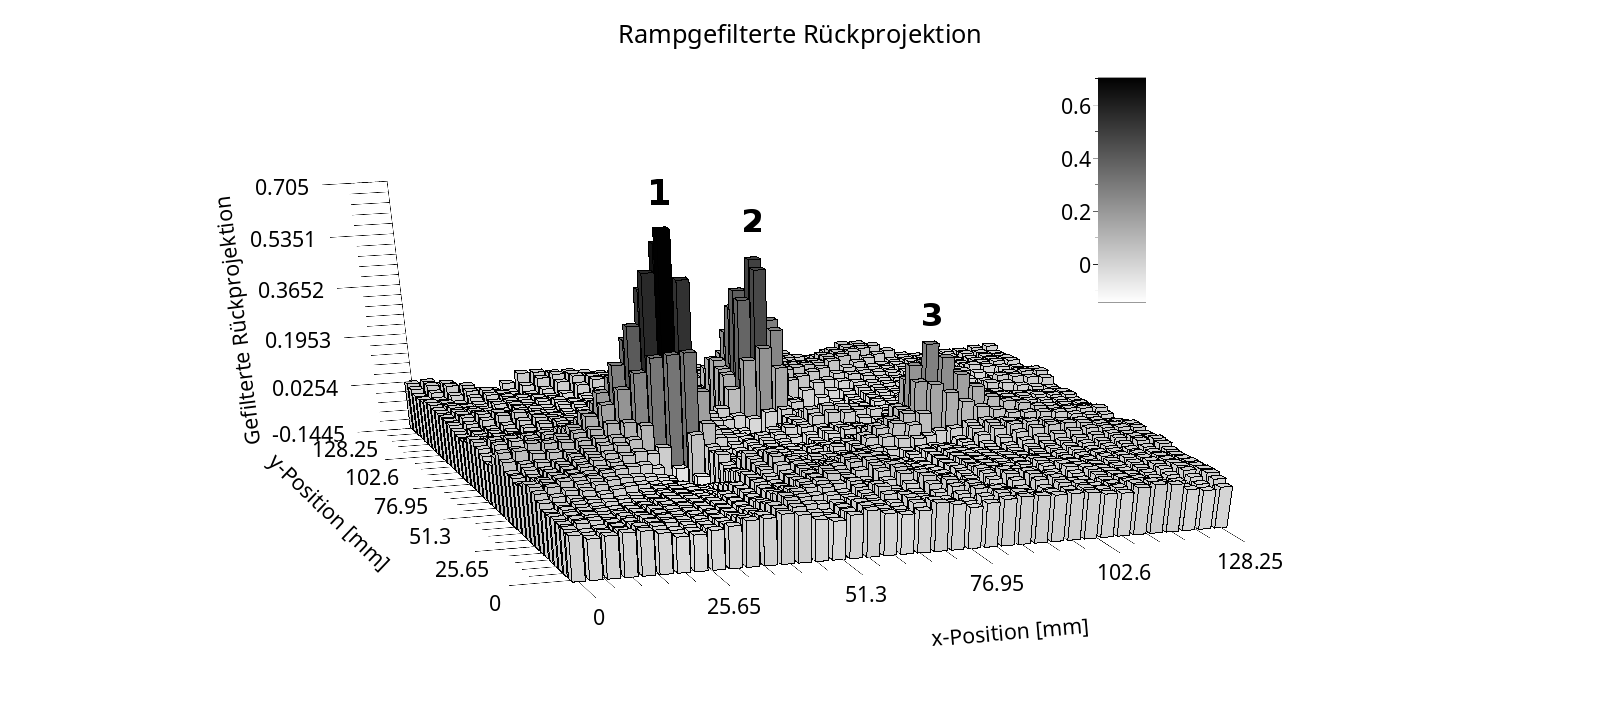
\includegraphics[width=2\textwidth, height=0.225\textheight]{pic/3dPlotTomographRamp.png}}
                                \label{dfd:Ramp}
                            \minipend
                            &
                            \hspace{3mm} 
                            \minipanf
                                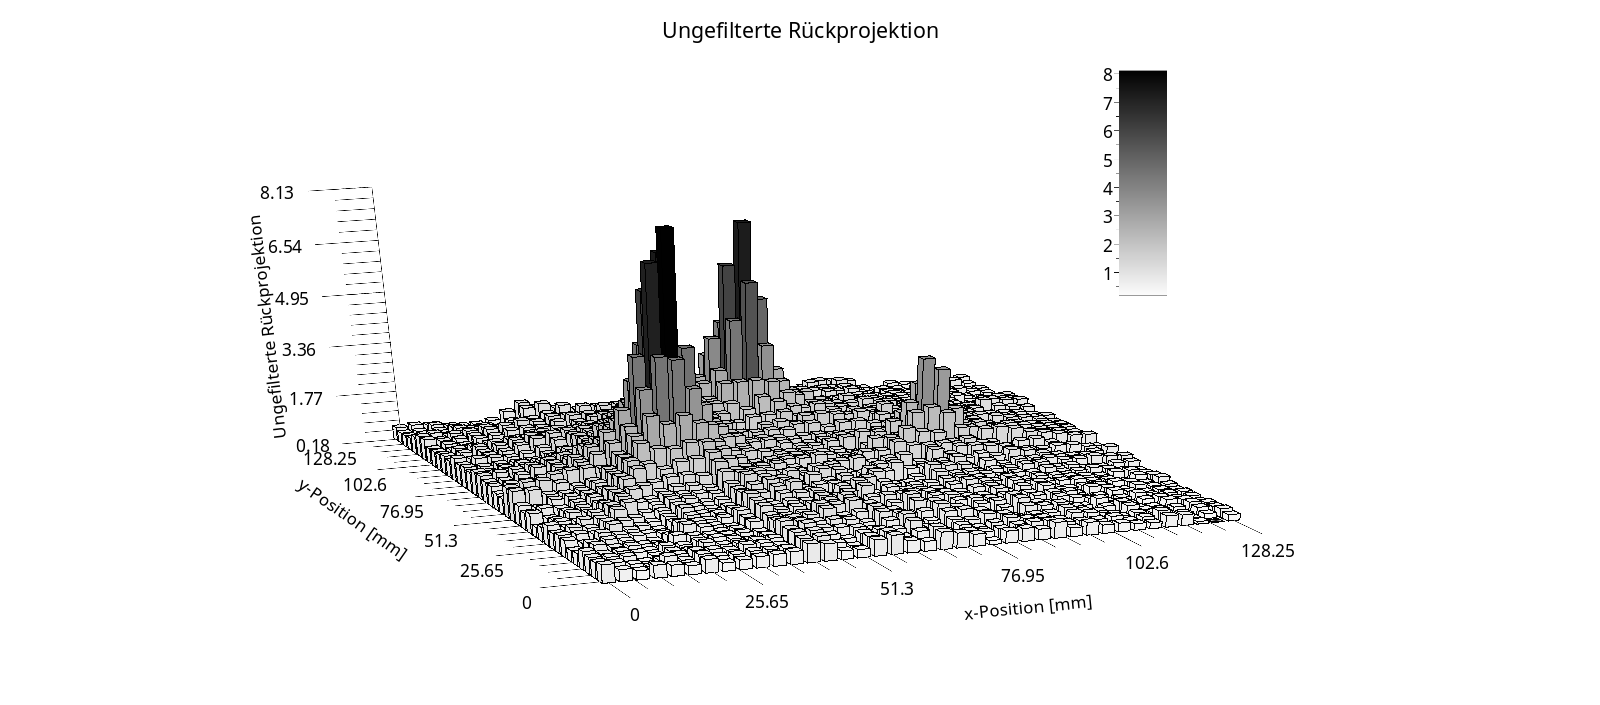
\includegraphics[width=2.2\textwidth, height=0.25\textheight]{pic/3dPlotTomographUngef.png}
                                \label{dfd:Ungefil}
                            \minipend \\               
             \end{tabular}
             \captionof{figure}{Gefilterte und Ungefilterte Rückprojektion der Aktivitätsverteilung}
            
            
            \textbf{Quantitative Auswertung}
            \begin{tabular}{cc}
                Zunächst wird die Position der 3 Quellen im verschlossenen Plastikbehältnis bestimmt. Dafür verwenden wir die in Abbildung (\ref{dfd:Ramp}) visualisierte Rückprojektion. 1 BIN des Rekonstruktionsrasters entspricht $3,375\ \unit{mm}$. Die Position der Quellen werden mit Hilfe der lokalen Maxima identifiziert.\\
                Anschließend quantifiziert man die Aktivität der Quellen, indem man über einen kleinen Bereich der rückprojizierten Verteilung um die Peaks mittelt. Es wurde in dieser Auswertung ein quadratischer Bereich um den Peak gewählt, in welchem Werte anzutreffen waren, die in der Nähe des FWHM (=Full Width Half Maximum) lagen. Dieses Vorgehen wird durch Abbildung (\ref{dfd:Mittelung}) visualisiert.
                &
                \hspace{3mm} 
                \minipanf
                	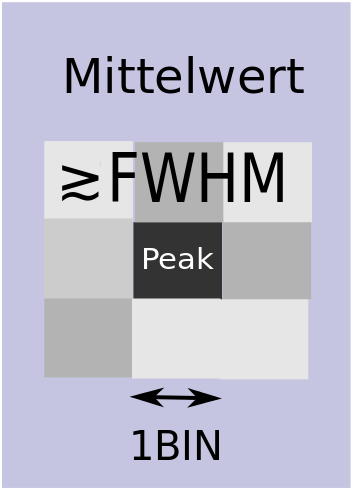
\includegraphics[width=2.2\textwidth, height=0.25\textheight]{pic/Skizze_Mittelung.png}
                	\label{dfd:Mittelung}
                \minipend \\               
            \end{tabular}
            
        \subsubsection{Messung einer Quellkonfiguration, Phantom isotroper Dichteverteilung}
          \textbf{Hauptversuch}\\
          Als nächsten wurde eine Messung mit unbekannter Quellverteilung gestartet. Die Energie- und das Zeitfenster entsprechen den oben bestimmten Intervallen.\\ \ \\
          \minipanf  
            \begin{center}
            \begin{tabular}{p{7cm}p{7cm}c}
                \textbf{ungefilterter Projektion} & \textbf{gefilterte Rückprpjektion}\\
                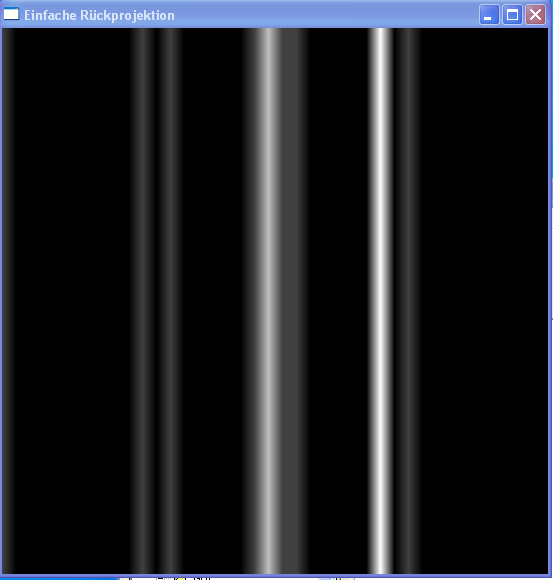
\includegraphics[width=0.3\textwidth, height=0.2\textheight]{pic/Einzelfenster_Bilder/unbekannte_Quelle/unbek1_einf_prj.png}
                & 
                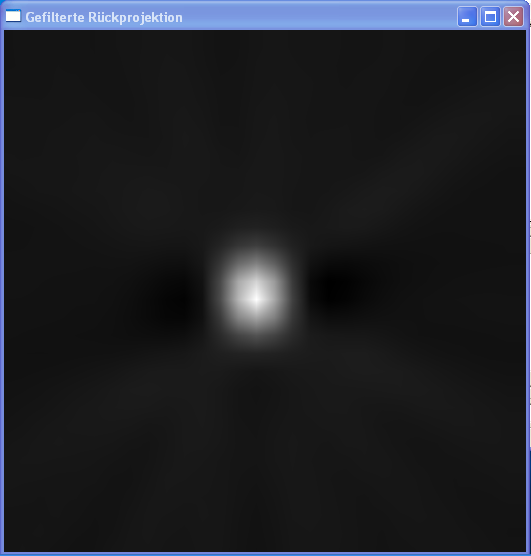
\includegraphics[width=.3\textwidth, height=0.2\textheight]{pic/Einzelfenster_Bilder/unbekannte_Quelle/unbek1gef_prj.png}\\
                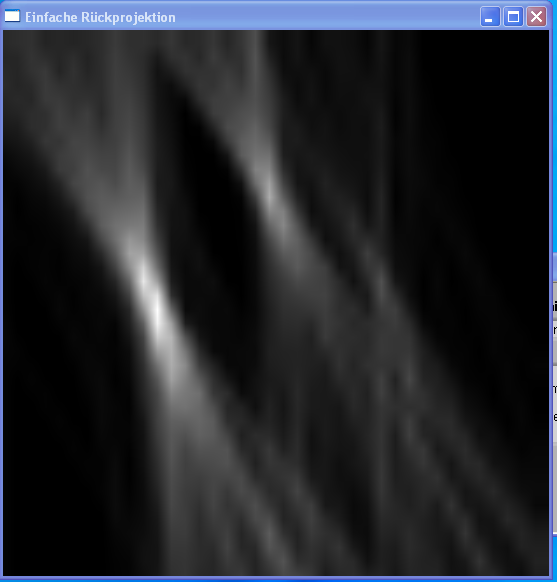
\includegraphics[width=0.3\textwidth, height=0.2\textheight]{pic/Einzelfenster_Bilder/unbekannte_Quelle/unbek2einf_prj.png}
                & 
                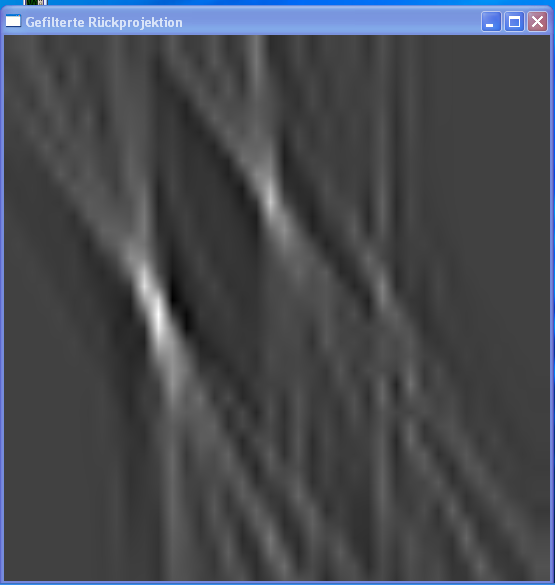
\includegraphics[width=.3\textwidth, height=0.2\textheight]{pic/Einzelfenster_Bilder/unbekannte_Quelle/unbek2gef_prj.png}\\ 
                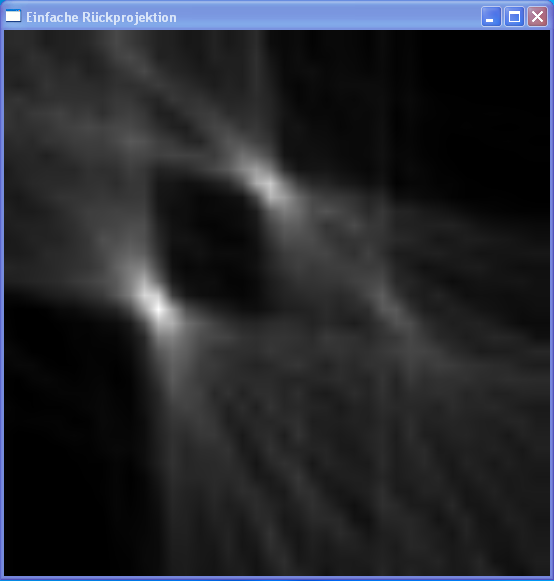
\includegraphics[width=0.3\textwidth, height=0.2\textheight]{pic/Einzelfenster_Bilder/unbekannte_Quelle/unbek3einf_prj.png}
                & 
                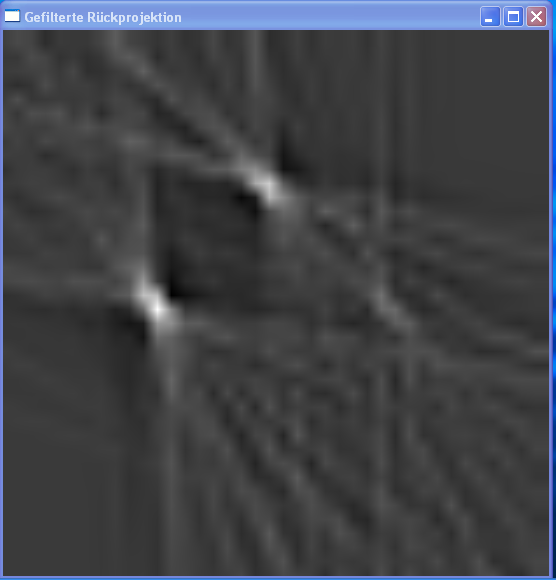
\includegraphics[width=.3\textwidth, height=0.2\textheight]{pic/Einzelfenster_Bilder/unbekannte_Quelle/unbek3gef_prj.png}\\               
                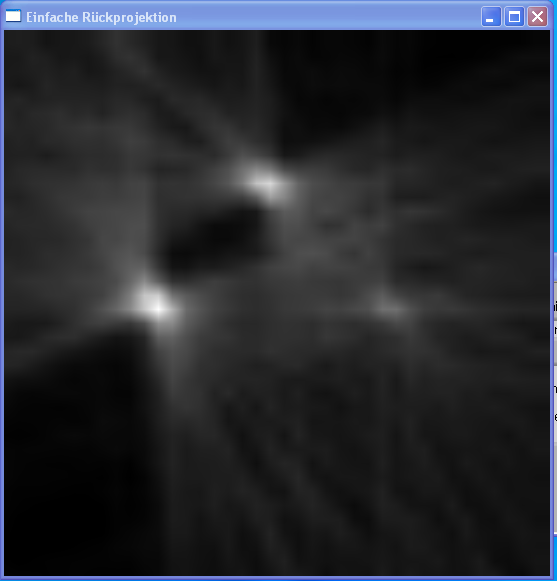
\includegraphics[width=0.3\textwidth, height=0.2\textheight]{pic/Einzelfenster_Bilder/unbekannte_Quelle/unbek4einf_prj.png}
                & 
                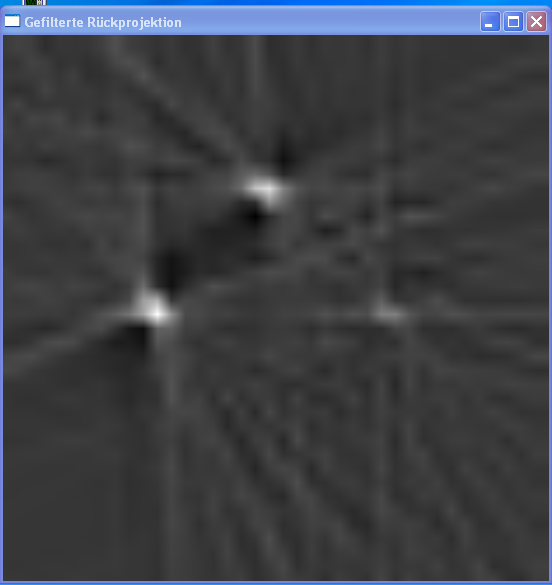
\includegraphics[width=.3\textwidth, height=0.2\textheight]{pic/Einzelfenster_Bilder/unbekannte_Quelle/unbek4gef_prj.png} \pagebreak
            \end{tabular}
            \captionof{figure}{Screenshots der Bildenstehung der gefilterten (rechts) und ungefilterten (links) Rückprojektion}
            \end{center}
          \minipend\\
          Test, Test %Notiz, bitte entfernen
            \textbf{Untersuchung des Einflusses verschiedener Filter}\\
          \minipanf  
              \begin{tabular}{p{4.5cm}p{4.5cm}p{4.5cm}c}
                  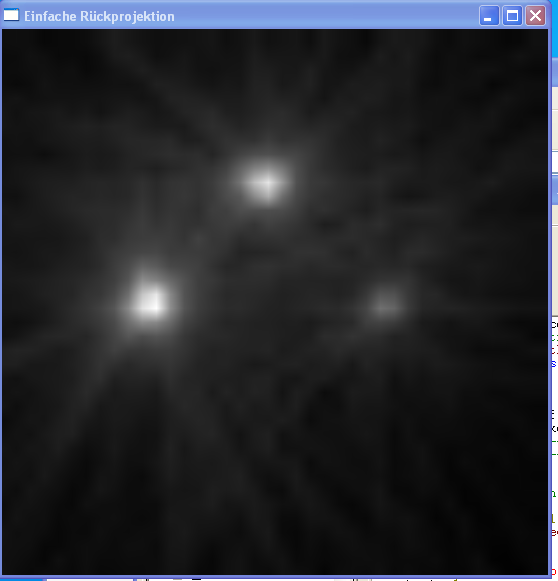
\includegraphics[width=0.25\textwidth, height=0.15\textheight]{pic/Einzelfenster_Bilder/unbekannte_Quelle/unbek5_einf_prj.png}
                  \captionof{figure}{ungefilterten Rückprojektion}
                  & 
                  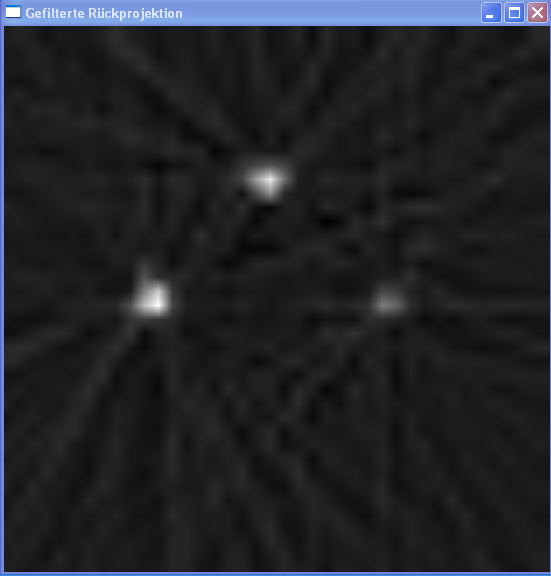
\includegraphics[width=.25\textwidth, height=0.15\textheight]{pic/Einzelfenster_Bilder/unbekannte_Quelle/unbek5_ramp.png}
                  \captionof{figure}{Rampf-Filter}
                  &
                  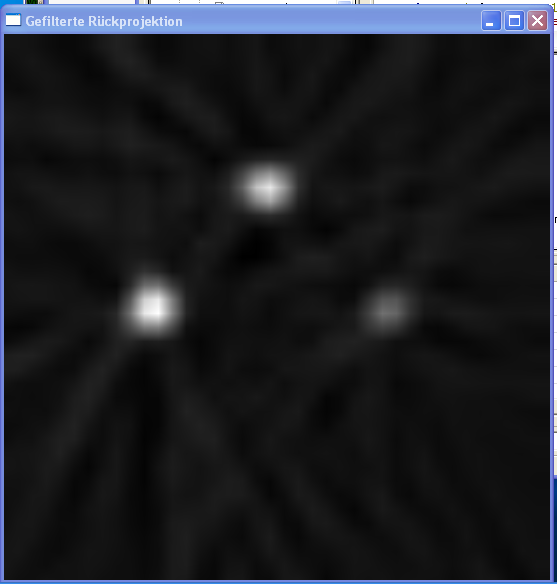
\includegraphics[width=0.25\textwidth, height=0.15\textheight]{pic/Einzelfenster_Bilder/unbekannte_Quelle/unbek5_hanning_weighted.png}
                  \captionof{figure}{Hanning-weighted-Filter}\\
                  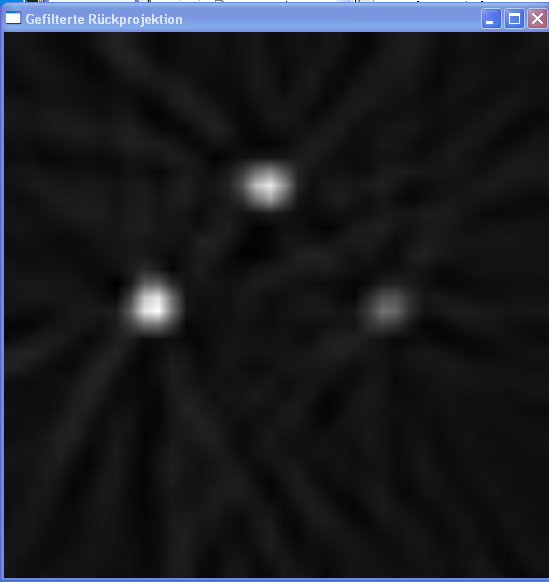
\includegraphics[width=.25\textwidth, height=0.15\textheight]{pic/Einzelfenster_Bilder/unbekannte_Quelle/unbek5_middle.png} 
                  \captionof{figure}{Middle-Filter}
                  &
                  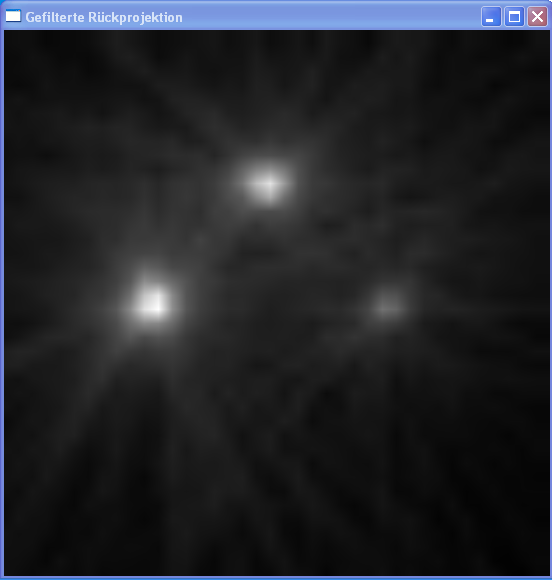
\includegraphics[width=0.25\textwidth, height=0.15\textheight]{pic/Einzelfenster_Bilder/unbekannte_Quelle/unbek5_rausch3.png}
                  \captionof{figure}{Rauschfilter bei Dimension 3}
                  & 
                  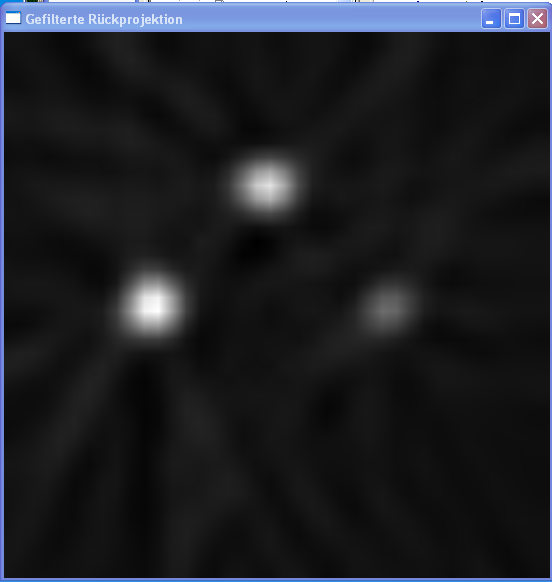
\includegraphics[width=.25\textwidth, height=0.15\textheight]{pic/Einzelfenster_Bilder/unbekannte_Quelle/unbek5_rausch13.png}               
                  \captionof{figure}{Rauschfilter bei Dimension 13} \pagebreak[2] 
                  \\
                  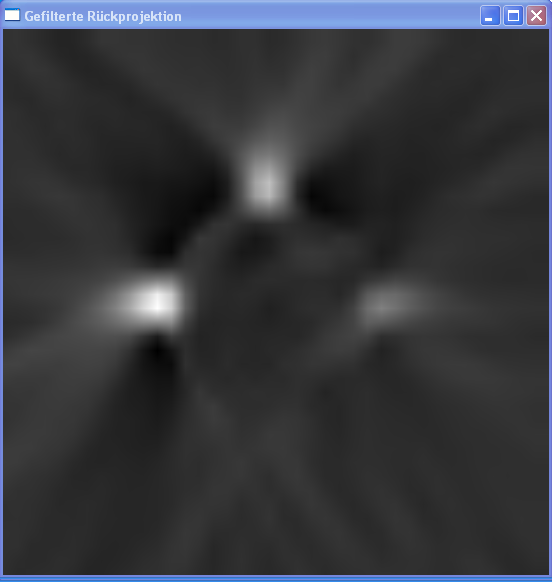
\includegraphics[width=0.25\textwidth, height=0.15\textheight]{pic/Einzelfenster_Bilder/unbekannte_Quelle/unbek5_rausch25.png}
                  \captionof{figure}{Rauschfilter bei Dimension 25}
                  &
                  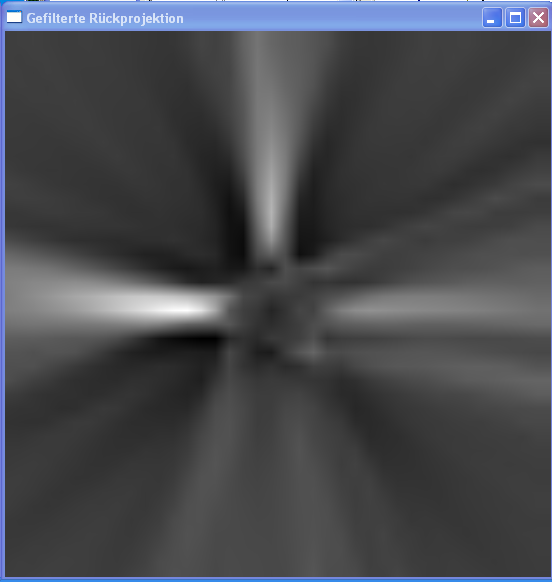
\includegraphics[width=.25\textwidth, height=0.15\textheight]{pic/Einzelfenster_Bilder/unbekannte_Quelle/unbek5_rausch36.png} 
                  \captionof{figure}{Rauschfilter bei Dimension 36}
                  &
                  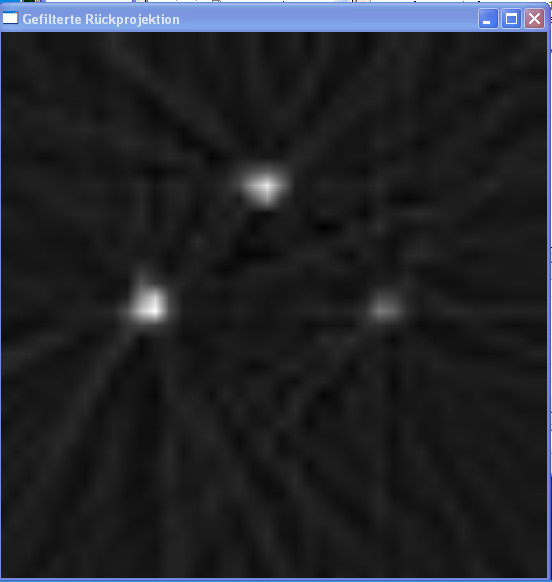
\includegraphics[width=.25\textwidth, height=0.15\textheight]{pic/Einzelfenster_Bilder/unbekannte_Quelle/unbek5_shepp-logan.png}
                  \captionof{figure}{Shepp-Logan-Filter}
                \end{tabular}\\
                Die Abbildungen drei bis elf zeigen die Anwendung verschiedener Filter auf die ungefilterte Rückprojektion, wobei der Standardwert der Dimension 13 ist
            
            \minipend\\ \ \\            
            
            
        \subsubsection{Messung mit einer Punktquelle, Phantom an-/insotroper Dichteverteilung}